\chapter{Gravitation and astrophysics}

\section{What goes up\ldots}

\subsection{Newton}

Gravity is one of the fundamental forces of nature; familiar as the force that keeps the Earth in orbit about the Sun and makes falling off a log so easy. \citet[book 3]{Newton1999} was the first to realise that gravitation could explain both apples falling from trees and the motion of astronomical bodies. In the \textit{Principia}, first published in 1687, he outlined a gravitational force that scaled as the inverse of the square of the distance between centres of mass and was proportional to the product of the masses of the bodies. In modern notation the force is
\begin{equation}
F = \frac{G m_1 m_2}{r^2},
\end{equation}
for distance $r$, masses $m_1$ and $m_2$, and gravitational constant $G$. This theory has been hugely successful. Not only is it still taught in schools today, but it is also used for astronomical research. Newton's law of universal gravitation has proved accurate in describing orbital motions. However, there have been observations that did not fit its predictions.

In the early nineteenth century, the motion of Uranus was found to deviate from its expected trajectory. Rather than seeking to modify the theory, \citet[\textit{troisi{\`e}me partie}]{LeVerrier1846} and \citet[papers 1 and 2]{Adams1896} calculated the properties of a perturbing object that could explain the motion. They predicted the existence of an unseen mass, a new planet; this was subsequently observed within a degree of Le Verrier's hypothesised position \citep[\textit{cinqui{\`e}me partie}]{LeVerrier1846} and became known as Neptune.

Newtonian gravity survived the trial of Uranus' orbit, but it could not explain the perihelion precession of Mercury. \citet[\textit{chapitre XV}, \textit{section quatri{\`e}me}]{LeVerrier1859} first noticed the anomaly. A new inner planet was suggested, but this time it could not be found. What was needed was a modified theory of gravitation: the Newtonian theory is insufficient in the stronger gravity close to the Sun \citep[document 24]{Einstein1997}.

\subsection{Einstein}

The new extended theory was General Relativity (GR), developed by Einstein in the 1910s \citep{Einstein1997}. This describes gravity as the effect of the curvature of spacetime, which is now a dynamical entity. Particles naturally travel along geodesics of spacetime, which may appear curved; the curvature of spacetime itself is sourced from the energy-momentum it contains: matter tells spacetime how to curve, and spacetime tells matter how to move \citep[section 1.1]{Misner1973}. This is encapsulated within the Einstein field equations \citep[documents 22 and 25]{Einstein1997}
\begin{equation}
R_{\mu\nu} - \recip{2}R g_{\mu\nu} = \frac{8\pi G}{c^4}T_{\mu\nu},
\end{equation}
where $g_{\mu\nu}$ is the metric, $R_{\mu\nu}$ and $R$ are the Ricci tensor and scalar (\citealt[section 8.7]{Misner1973}; \citealt[section 3.2]{Wald1984}), $c$ is the speed of light, and $T_{\mu\nu}$ is the energy-momentum tensor. GR reduces to its Newtonian counter-part in the weak-field limit, or conversely, it extends Newtonian gravity to stronger gravitational fields.

Since its inception, GR has successfully passed every observational test \citep{Will1993, Will2006}. However, astronomers have not been idle, and the twentieth century has yielded further surprises.

Observations of the velocity dispersions of galaxies in clusters are higher than those calculated from the quantity of luminous matter \citep[e.g.,][]{Zwicky1937}. Similarly, measurements of the rotation curves of galaxies do not match the expected profile \citep{Babcock1939}. Gravitational lensing of galaxy clusters confirms that their gravity is dominated by an unseen component \citep{Bergmann1990,Clowe2006}. This has been interpreted as motivation for introducing dark matter, a new component of the Universe that gravitates but does not interact with electromagnetic radiation. Dark matter has become central to our understanding of cosmology \citep[e.g.,][]{Springel2006a}; it is needed to explain structure formation: without it we could not form galaxies from the small over-densities inferred from the homogeneity of the cosmic microwave background \citep{White1978,Liddle1993}. Although we know the properties required of dark matter and we can estimate the required quantity, we do not have a definite candidate for a dark matter particle \citep{Bertone2005}. Its true nature remains a mystery.

Observations of type IA supernovae have revealed that the Universe is not only expanding, but is accelerating \citep{Riess1998,Perlmutter1999}. This acceleration has been attributed to the influence of dark energy \citep{Perlmutter1999a,Peebles2003}. The nature of dark energy is even more mysterious than that of dark matter. The simplest explanation is to introduce a cosmological constant $\Lambda$; this modifies the Einstein field equations to become \citep[document 43]{Einstein1997}
\begin{equation}
R_{\mu\nu} - \recip{2}R g_{\mu\nu} - \Lambda g_{\mu\nu} = \frac{8\pi G}{c^4}T_{\mu\nu}.
\end{equation}
This model has been highly successful in explaining the evolution of the Universe, but we still do not know if a cosmological constant is the true explanation and if so, why it has its particular value \citep{Carroll2001}.

Despite its long history, we still do not know everything about gravity. There are still discoveries to be made. Gravity is the weakest of the fundamental forces and so is difficult to study in the laboratory. Yet it dominates on astronomical scales; understanding gravity is crucial to understanding the cosmos. We have learnt much about the workings of the Universe through improving our understanding of gravity, and the motivation for developing new theories of gravitation has often come from astronomical observations. Gravitation and astrophysics are intimately linked.

\subsection{This work}

This thesis is divided into two strands. The first is concerned with what we could learn about astrophysical systems from gravitational probes; the second is concerned with what we can learn about gravity from astronomical observations.  We shall consider strong-field tests and in particular gravitational waves. The former part concentrates on what we could hope to learn about massive black holes and their surrounding stellar environment from extreme-mass-ratio bursts. The latter looks at modifications to gravity in the metric $f(R)$ theory.

\section{Strong-field tests \& gravitational waves}

The deviations from Newtonian theory were first noted in the gravitational field close to the Sun, the strongest accessible in the Solar System. GR has now been tested in stronger fields \citep{Will2006}, but there are still more extreme systems to be explored. It is here that we would expect any deviations to manifest. We know at least that our understanding of GR in the strongest fields is incomplete, as black holes feature singularities at their centres, where the theory breaks down (\citealt[section 34.6]{Misner1973}; \citealt[chapter 9]{Wald1984}). Even if we do not find any deviations from GR, it is still worthwhile to check its validity, if only as a matter of scientific principle.

\subsection{Field strength \& existing tests}

In order to parametrize the strength of gravity, \citet{Psaltis2008a} introduces two characteristic quantities: the dimensionless potential or compactness \citep{Yunes2013}
\begin{equation}
\varepsilon = \frac{GM}{rc^2},
\end{equation}
and the dimensionful curvature
\begin{equation}
\xi = \frac{GM}{r^3c^2},
\end{equation}
where $M$ is the gravitating mass and $r$ a characteristic distance. These are larger for stronger fields. The potential ranges from $\varepsilon \simeq 0$ in weak fields to $\varepsilon = \order{1}$ at a black hole event horizon. It is useful in defining post-Newtonian expansions. The curvature $\xi$ approximates the form of the Ricci scalar, which is fundamental to GR. It is necessary to pick a particular reference scalar to define when the curvature becomes large; however, it is a useful gauge of the strength of a gravitational field in a geometric theory, because it is the lowest order measure that cannot be eliminated by a coordinate transformation \citep[chapter 7]{Hobson2006}.

Using these two parameters, we can map out the possible tests of GR. \Figref{Psaltis} shows a selection of current astrophysical tests.
\begin{figure}
  \begin{center}
  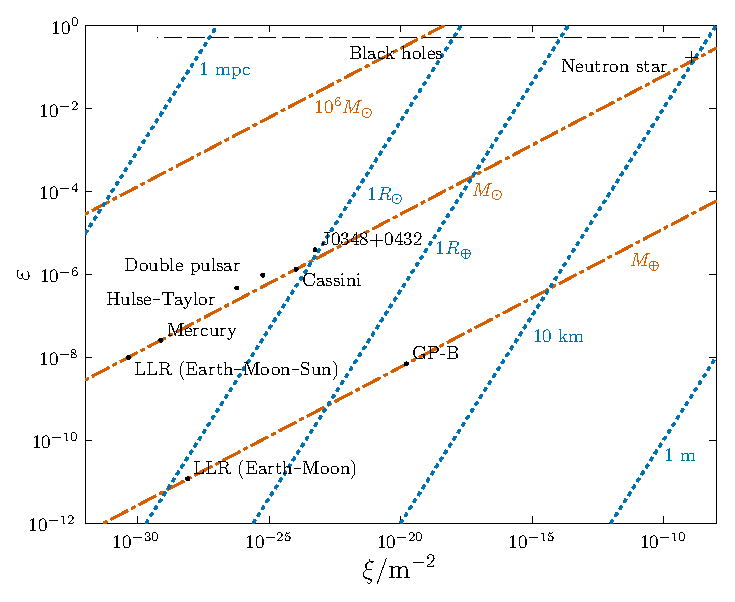
\includegraphics[width=0.6\textwidth]{./images/Fig_Psaltis_plot}
    \caption{Astrophysical tests of GR parametrised by the compactness and curvature scales they probe, adapted from \citet{Psaltis2008a}. The dashed line indicates the Schwarzschild radius $r\sub{S} = 2 GM /c^2$ for black holes of mass $5$--$10^7M_\odot$ and the cross indicates the surface of a neutron star.}   
    \label{fig:Psaltis} 
  \end{center}
\end{figure}
Included are:
\begin{itemize}
\item The classic perihelion precession of Mercury (\citealt[section 10.2]{Hobson2006}; \citealt[section 7.3]{Will1993}; \citealt{Pitjeva2009a});
\item Doppler tracking of the Cassini spacecraft \citep{Bertotti2003} which measures the time delay of light travelling past the Sun \citep[section 7.2]{Will1993};
\item Lunar laser ranging (LLR; \citealt{Bender1973,Williams2012}) which provides precise measurements of the orbits of the Earth--Moon and Earth--Moon--Sun systems \citep[section 8.1]{Will1993};
\item Gravity Probe B (GP-B; \citealt{Everitt2009,Everitt2011}) measurements of the geodetic drift and frame-dragging \citep[section 9.1]{Will1993};
\item A selection of binary pulsars \citep{Taylor1993,Stairs2003}, specifically the Hulse--Taylor binary (PSR B1913+16; \citealt{Hulse1975,Weisberg2010}), which was the first discovered and the first system to show the influence of gravitational waves; PSR J0348+0432 \citep{Antoniadis2013} which includes a $2 M_\odot$ pulsar, and the double pulsar system \citep{Breton2008,Kramer2008}. % PSR B1534+12 \citep{Stairs2002};
\end{itemize}
For comparison, we have also plotted the parameters for the surface of a neutron star and the Schwarzschild radius of black holes of various masses. Black holes range in mass from a few solar masses \citep{Ozel2010} to several billion solar masses \citep{Hlavacek-Larrondo2012}, although, for clarity, we have only plotted up to $10^7 M_\odot$. To probe the strongest fields, we need a way of probing the spacetime of compact objects like neutron stars and black holes.

In addition to the astrophysical tests of gravity, it is possible to make precision tests in the laboratory \citep{Kapner2007a,Adelberger2009,Wagner2012}. Whilst these are limited to using small masses, they do allow careful control of the system that is not possible in astronomy. Neither the astrophysical nor the laboratory tests performed so far show any discrepancy from the predictions of GR \citep{Will2006}. 

\subsection{Gravitational radiation}

One particularly promising method of exploring strong-field regions would be to observe gravitational waves (GWs). These are predicted in any relativistic theory of gravity, where changes in the gravitational field must propagate at finite speed \citep{Schutz1984}. Within GR they are tiny ripples in the spacetime metric (\citealt[section 35.1]{Misner1973}; \citealt[section 107]{Landau1975}). They are generated by systems with a time-varying mass quadrupole; significant gravitational radiation originates from regions where spacetime is highly dynamic and the objects are extremely relativistic. This is precisely the strong-field domain we are interested in investigating.

Some intuition about GWs can be obtained from the more familiar electromagnetic (EM) waves (\citealt[sections 46--48 and 66--67]{Landau1975}; \citealt[sections 7.1 and 9.1--9.3]{Jackson1999}). These are oscillations of the electric and magnetic fields produced by accelerating charges whilst GWs are oscillations of spacetime produced by accelerating masses. EM waves may be sourced by a time-varying charge dipole; as a consequence of conservation of momentum there is no time-varying mass dipole, so GWs are sourced by the mass quadrupole (\citealt[section 18.5]{Hobson2006}; \citealt[section 15.4]{Rindler2006}). Both waves propagate at the speed of light and have two (transverse) polarizations: for GWs these represent two orthogonal patterns of stretching and squeezing as shown if \figref{plus-cross} (\citealt[section 34]{Dirac1996}; \citealt[section 18.4]{Hobson2006})
\begin{figure}
  \begin{center}
  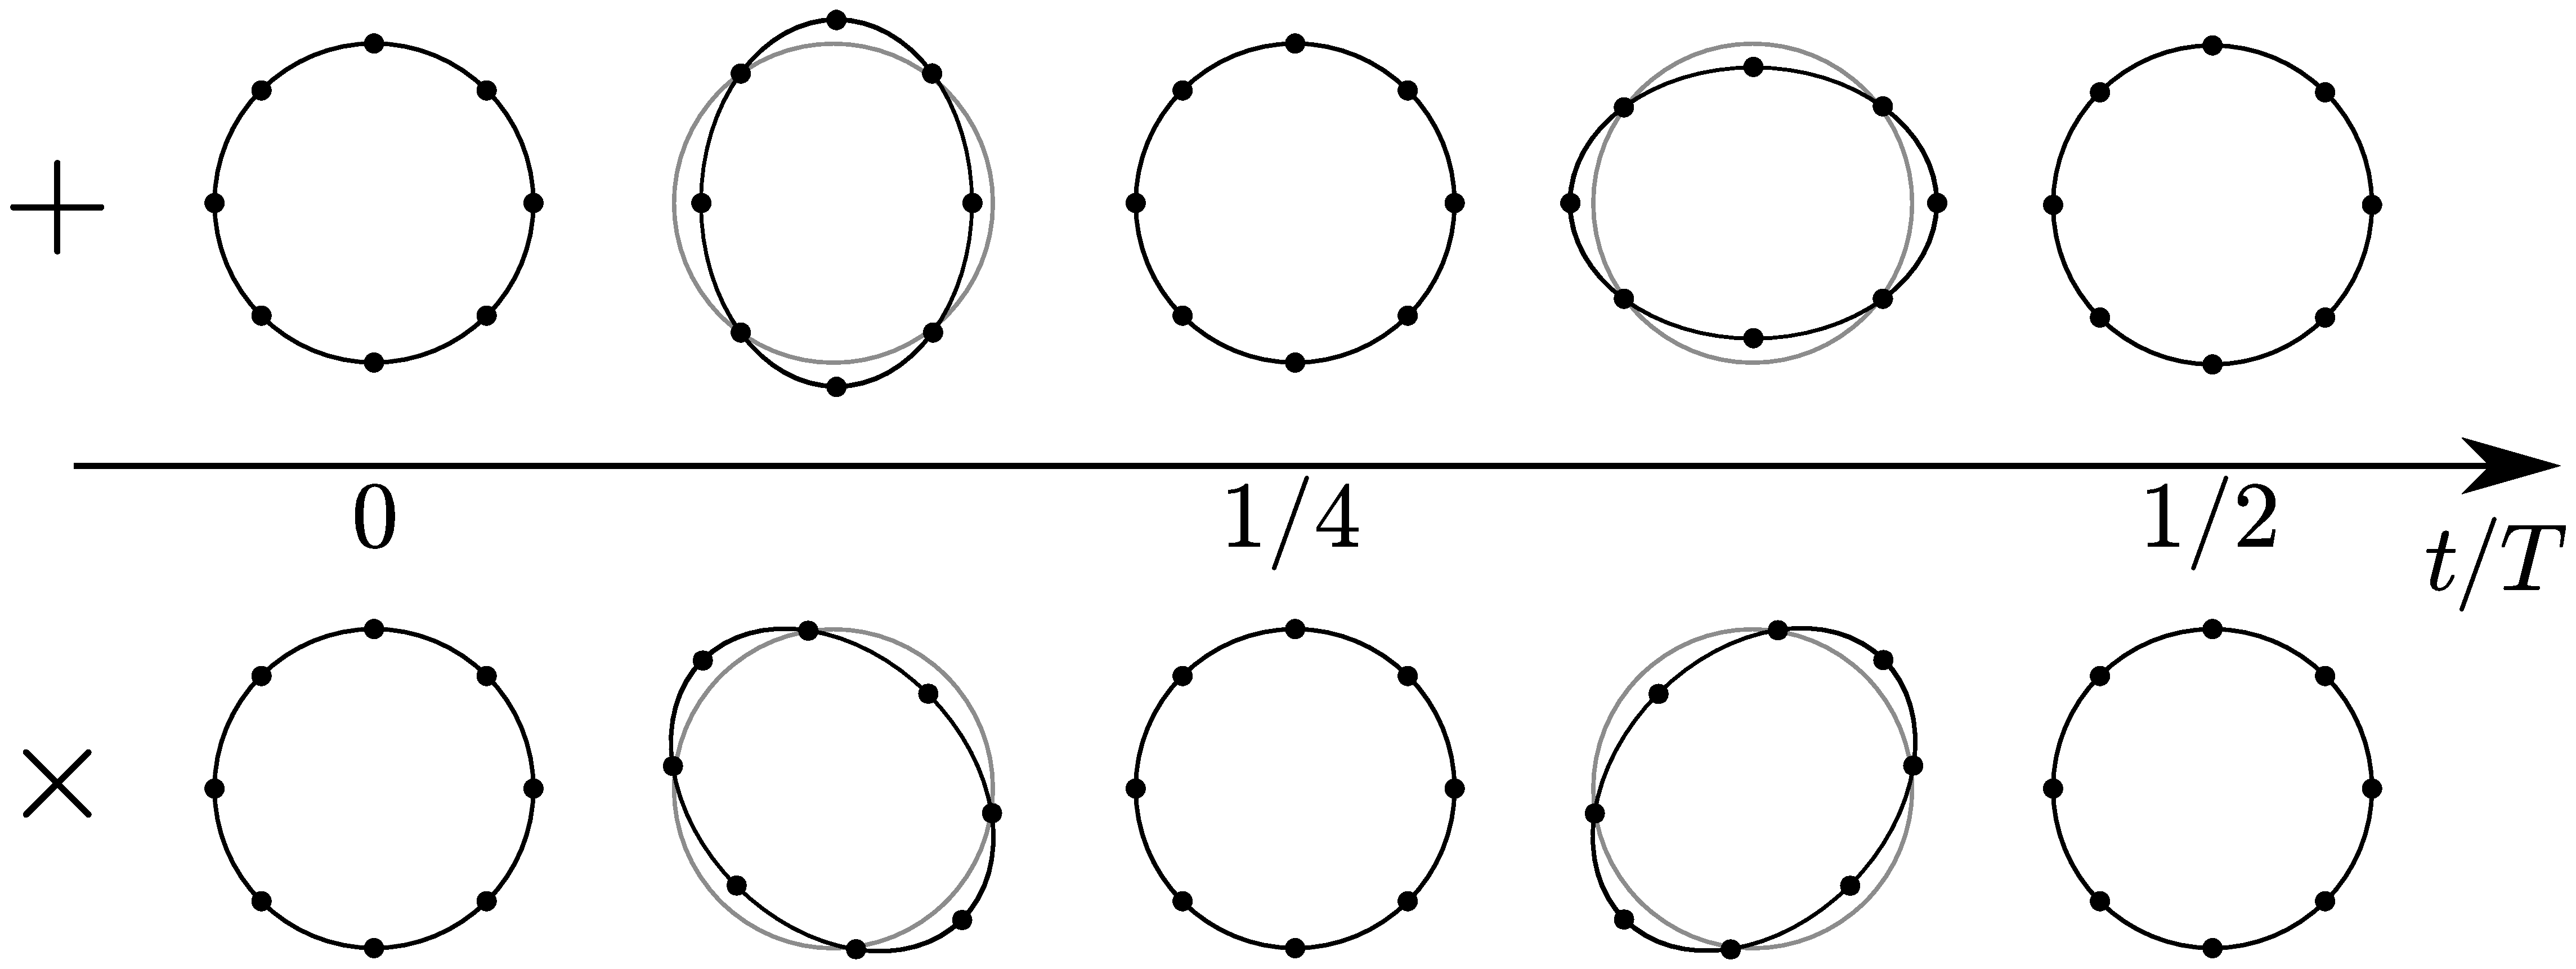
\includegraphics[width=0.65\textwidth]{./images/Polarization}
    \caption{The effect the two GW polarizations (plus $+$ and cross $\times$) on a ring of free particles as a function of time. The propagation direction is perpendicular to the ring. The wave period is $T$.}   
    \label{fig:plus-cross} 
  \end{center}
\end{figure}

Visible light has been used by astronomers for millennia. In the twentieth century, the useful spectrum was extended through infrared to radio, and from ultraviolet to X-rays and gamma rays \citep[chapter 7]{Longair2006}. In the twenty-first century, we hope to move from EM radiation to gravitational radiation as a tool for astronomy. GWs encode valuable information about their sources, information that is accessible by other means.

Just like EM waves, GWs come in a range of frequencies. The frequency is set by the scale of the source system: typically more massive objects have longer associated timescales and so produce lower frequency radiation. \Figref{spectrum} show the GW spectrum with illustrative detectors and sources.
\begin{figure}
  \begin{center}
  %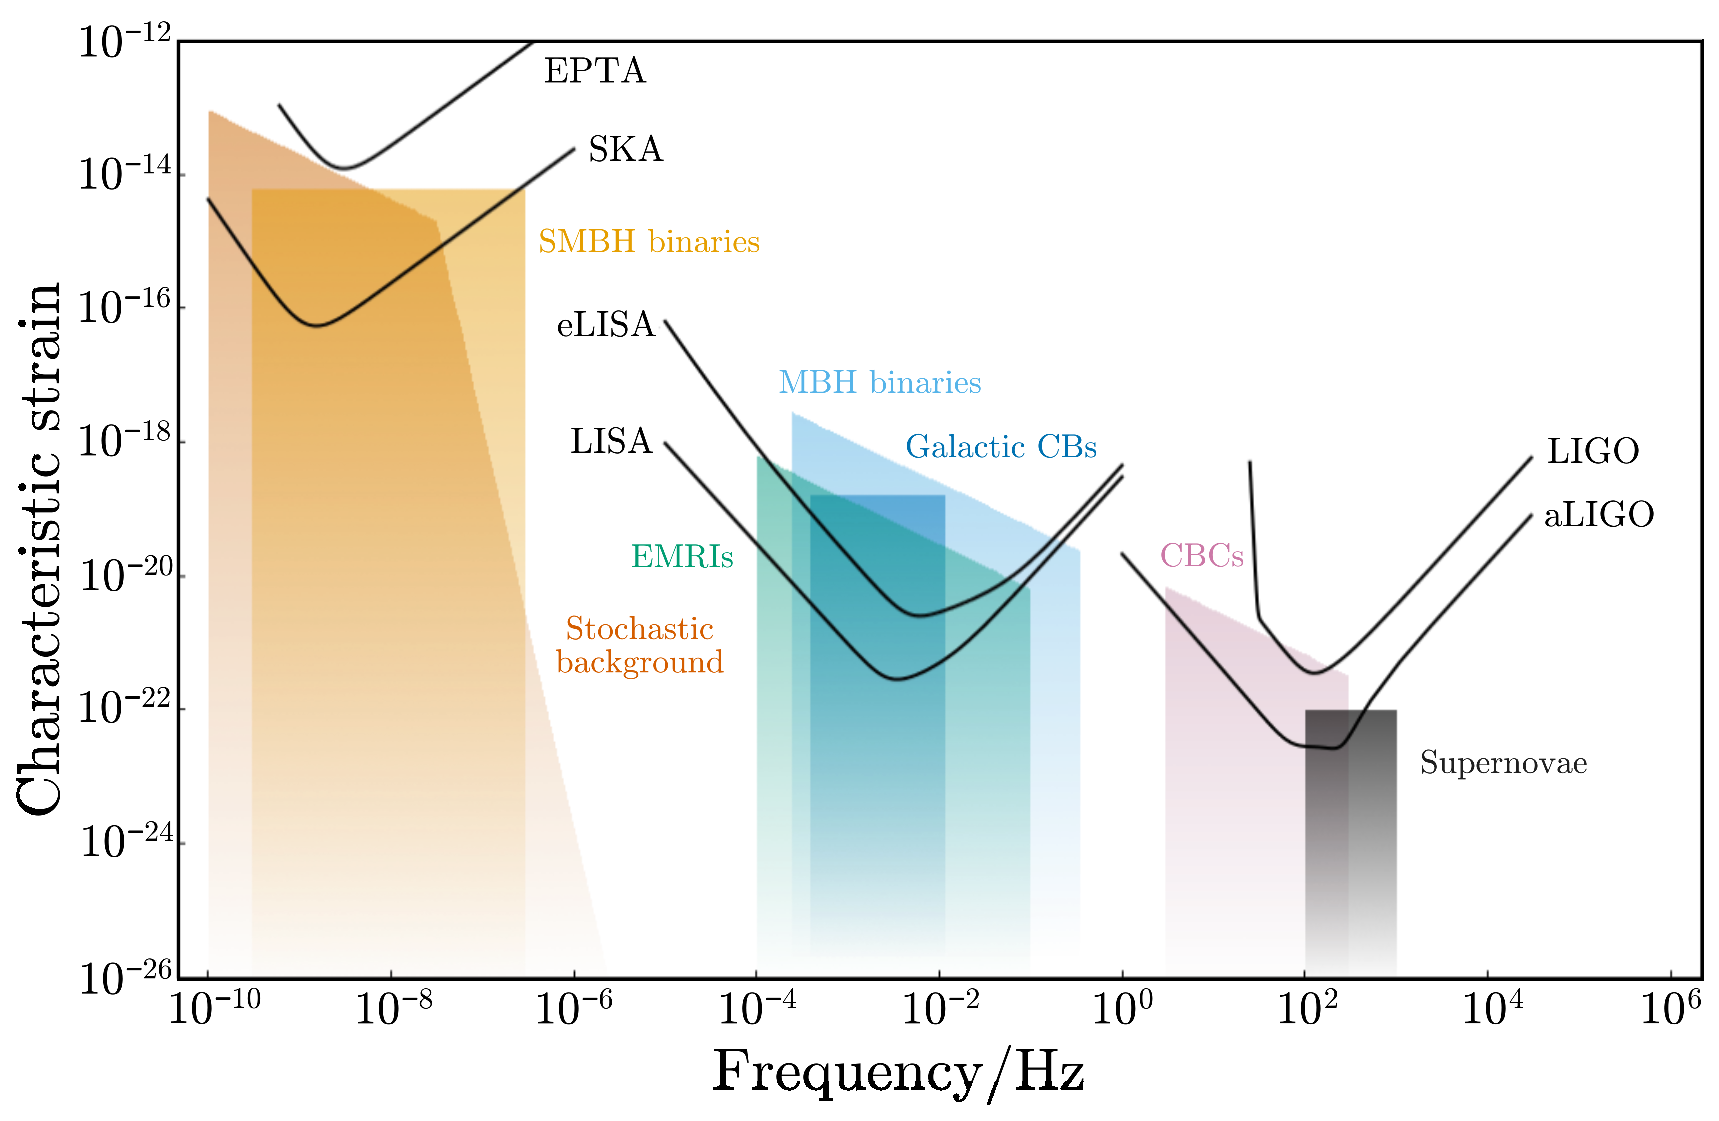
\includegraphics[width=0.95\textwidth]{./images/GW_spectrum}
    \caption{The spectrum of GWs. Sources are indicated by their characteristic amplitude as measured on Earth, detectors are characterised by their sensitivity curves.}   
    \label{fig:spectrum} 
  \end{center}
\end{figure}
Detectors are sensitive to specific frequency bands, the range of which is set by their scale. The spectrum may be divided into: the extremely low frequency (ELF; not shown in the figure) regime, $\sim10^{-18}$--$10^{-15}\units{Hz}$, which may indirectly detected through observations of the polarization of the cosmic microwave background (CMB; \citealt[e.g.,][]{Hu1997,Kamionkowski1997}); the very low frequency (VLF) regime, $\sim10^{-9}$--$10^{-6}\units{Hz}$, which is accessible to pulsar timing arrays (PTAs); the low frequency (LF) regime, $\sim10^{-6}$--$1\units{Hz}$, which could be measured by space-borne detectors, and the high frequency (HF) regime, $\sim1$--$10^4\units{Hz}$, which is the target range for ground-based detectors. Individual detectors are discussed in \secref{GW-det} and some example sources are introduced in \secref{GW-sources}.

While GWs are an exciting source of information, it will be beneficial to compare with results from other techniques, to maximise the data available for inferences, and to check models. For example, very long baseline interferometry (VLBI) may be used to image the vicinity of a BH's horizon, or X-ray observations could be used to investigate BH accretion discs \cite{Psaltis2008}.

\subsubsection{Gravitational wave detection}\label{sec:GW-det}

As yet no GWs have been directly detected, although their existence has been inferred from the loss of energy and angular momentum from binary pulsars \citep{Stairs2003}. ... There are a number of experiments designed to directly observe GWs \citep{Riles2012}. Modern detectors attempt to measure the minute changes in distance induced by a passing GW (\citealt[section 9.5]{Thorne1987}; \citealt[section 18.9]{Hobson2006}). The amplitude of a GW is characterised by a strain: the fractional change in length resulting from the perturbation from the background spacetime.

The Laser Interferometer Gravitational-wave Observatory (LIGO; \citealt{Abramovici1992}) and the European Gravitational Observatory's Virgo detector \citep{Acernese2008a}, which work in collaboration, are currently being upgraded to their advanced configurations and are expected to make the first detection shortly after recommencing operation around 2015 \citep{Harry2010,Accadia2011}.\footnote{An optimistic hope is to celebrate the centenary of Einstein's 1916 prediction of gravitation waves \citep[document 32]{Einstein1997} with the first direct detection.} These are ground-based interferometers that detect passing GWs by measuring the induced difference in the length of their two arms \citep{Pitkin2011}. They are sensitive to frequencies in the range $\sim10$--$10^4\units{Hz}$, with peak sensitivity at about $100\units{Hz}$. The LIGO and Virgo detectors are supported by GEO 600, a smaller interferometric experiment that incorporates prototype technologies \citep{Willke2002,Willke2006}. LIGO has two sites, one in Hanford, Washington and one in Livingstone, Louisiana. The Hanford observatory has two detectors, one half the arm-length of the other. There is an agreement to move the smaller detector to a location in India \citep{Unnikrishnan2013}. The LIGO-India detector, operated by the Indian Initiative in Gravitational Observations (IndIGO), will provide a longer baseline between detectors, giving improved sky location and sky coverage \citep{Schutz2011}.

A further ground-based interferometer is under construction in Japan. The Kamioka Gravitational Wave Detector (KAGRA), formerly the the Large-scale Cryogenic Gravitational Wave Telescope (LCGT; \citealt{Kuroda1999,Kuroda2010}) will operate underground in the Kamioka mine. It lags several years behind the other detectors, but will employ more sophisticated noise-reduction techniques such as cryogenic cooling.

Ground-based GW astronomy may eventually be continued by the construction of the Einstein Telescope, an ambitious idea to construct an underground detector with $10\units{km}$ arms \citep{Punturo2010,Hild2011,Sathyaprakash2012}. Its location would provide shielding from seismic noise, allowing it to observe frequencies $10$--$10^4\units{Hz}$. There is no definite time-line for this concept.

There is another contender for the first detection: pulsar timing arrays \citep{McWilliams2012,Sesana2012a}. These infer the presence of a GW from periodic delays in the arrival times of the highly regular millisecond pulses. In effect, the pulsars are used to create a detector with galactic-scale arms. They are sensitive to frequencies of $\sim10^{-9}$--$10^{-7}\units{Hz}$. An international collaboration of European, North American and Australian radio telescopes is already in possession of the necessary instruments to detect GWs \citep{Hobbs2010}.\footnote{The International Pulsar Timing Array (IPTA) consortium consists of the European Pulsar Timing Array, the (North American) NANOGrav and the (Australian) Parkes Pulsar Timing Array consortia.} The completion of the Square Kilometre Array (SKA; \citealt{Dewdney2009}) shall augment the search, greatly increasing sensitivity \citep{Kramer2004}.

Between the high frequency range of the ground-based detectors and the very low frequency range of pulsar timing, lies a band that could be accessible to space-based interferometers. These are not limited by seismic noise and are free to have much longer arms than the ground-based detectors, making them sensitive to low frequencies. The paradigm detector is the Laser Interferometer Space Antenna (LISA; \citealt{Bender1998, Danzmann2003}). This is a constellation of three satellites in a circular, heliocentric orbit forming a three-armed interferometer. Each arm is $5 \times 10^9\units{m}$, and the orbit trails $20^{\circ}$ behind the Earth. The detector is sensitive to a range of frequencies $\sim10^{-5}$--$1\units{Hz}$, having peak sensitivity around $10^{-3}$--$10^{-2}\units{Hz}$.

LISA developed as a joint NASA--ESA mission. In 2011 NASA withdrew for financial reasons leaving ESA to investigate reduced cost missions. The resulting descoped concept is the evolved Laser Interferometer Space Antenna (eLISA; \citealt{Jennrich2011, Amaro-Seoane2012a}).\footnote{This was submitted to the ESA for their L1 mission selection as the New Gravitational-wave Observatory (NGO).} This shares the same basic components as LISA but only has two arms and lags $9^{\circ}$ behind the Earth. The arms are $1 \times 10^9\units{m}$; this shifts the peak sensitivity to marginally higher frequencies, around $10^{-2}\units{Hz}$. Overall the noise curve is raised relative to LISA giving eLISA reduced sensitivity.

At the time of writing, there is no currently funded mission. However, LISA Pathfinder, a technology demonstration mission, is due for launch in 2015 \citep{Anza2005, Antonucci2012}. Hopefully, a full mission shall follow in the subsequent decade.

In addition to the LISA family, there are other proposed space-borne detectors. The Japanese Deci-hertz Interferometer Gravitational Wave Observatory (DECIGO; \citealt{Kawamura2006,Kawamura2011}) consists of constellations of satellites similar to LISA, but with arms of $100\units{km}$. It will fill the gap between the LISA family and the ground-based detectors, being most sensitive to frequencies $0.1$--$10\units{Hz}$. DECIGO is imagined for launch in 2027 pending the success of two pathfinder missions \citep{Ando2010}.

There have even been suggestions for successors to LISA \citep{Crowder2005}. The Advanced Laser Interferometer Antenna (ALIA) and the Big Bang Observer (BBO) are both popular concepts. Compared to the LISA family, they have shorter arms, making them sensitive to higher frequencies, and better sensitivities. They may be more comparable to DECIGO \citet{Yagi2011a}. Since these designs are highly speculative, we shall not discuss them further.

\subsubsection{Gravitational wave sources}\label{sec:GW-sources}



Galactic compact binaries: Compact binaries are made up of at least one white dwarf or neutron star which orbits close to its companion. Such sources are so common in the Galaxy that they may begin to form a background of noise. Observations of these sources will help us to understand stellar population models and the evolution of stars. Some known Galactic binaries, called verification binaries, should be detectable within a few hours of operation of a space-borne detector, and will allow us to test that it is working. The binary systems slowly inspiral as gravitational waves carry away energy and momentum. Eventually the two objects merge. Neutron star-neutron star mergers are a potential candidate for short gamma rays bursts, one of the most energetic processes in the Universe.

Black hole mergers: One of the ways that galaxies evolve is through mergers. There is evidence to suggest that a supermassive black hole (SMBH), a black hole with a mass of over a million times the mass of the Sun, lurks at the centre of most galaxies. When two galaxies merge, the SMBHs in their centres can also spiral in together. The gravitational radiation emitted when they collide will be some of the loudest events in the Universe. More energy is emitted as gravitational radiation from one SMBH merger than as light from all the stars in the visible Universe. Measuring these mergers would tell us many interesting things about the properties of black holes, allowing us to test our understanding of GR, as well as informing our understanding of galaxy evolution.

Extreme-mass-ratio inspirals: In the core of galaxies, compact objects such as white dwarfs, neutron stars or black holes, may travel towards the SMBH at the centre of as a consequence of scattering form other objects. If they get close enough, they will start to inspiral as their orbits shrink due to the loss of energy and angular momentum carried away by gravitational waves. These are known as extreme-mass-ratio inspirals (EMRIs) on account of the huge difference in mass between the SMBH and the orbitting compact object. The inspiral is slow, meaning that we can observe gravitational waves emitted over hundreds of thousand of orbits. This allows us to build up an immensely detailed picture of the spacetime of the SMBH. These events would allow us to do fundamental physics by probing precisely the strong gravitational field about the SMBH, and, should we observe enough, we will be able to learn more about the stellar systems in the centre of galaxies.

The Big Bang: When the Universe was very young it underwent a period of very rapid expansion. Tiny fluctuations in spacetime would have been greatly stretched during this period and could still exist today as a background of gravitational waves. This could be detected by studying the polarisation patterns in the cosmic microwave background (CMB). With current instruments it is unlikely, but not impossible that we shall be able to measure the background. However, a positive detection would allow us to better understand the mechanism that drove early inflation of the Universe and probe extremely high energy physics. The gravitational wave background would allow us to see right back to the Big Bang, much further than we can see using EM radiation.

Phase transitions: As the Universe evolves from its early state it goes through a number of phase transitions which can be associated with symmetry breaking or decoupling of forces. These transitions can create lead to several different types of gravitational radiation. As an analogy, imagine cooling water so that it begins to form ice. This is a phase transition too. Ice begins to form as small crystals that grow outwards. The same can happen in the Universe, small pockets undergo the transition and these expand out as a bubble. For certain types of transitions, gravitational waves would be emitted when bubbles collide. In other cases, topological defects are created following the transition. The analogy would be when two crystals of ice grow together, but their structures are not quite aligned, so that that there is a clear boundary, a defect or domain wall. For spacetime, two examples of topological defects are cosmic strings and domain walls; the former are 1D strings of cosmic length, whereas domain walls are 2D. Such defects are expected to be rare as they have been diluted in space by the expansion of the Universe. However, they have a unique gravitational wave signal, which should make them easy to identify. Such a detection would be an exciting discovery of exotic physics.

...
...

\section{Astrophysical compact objects}

To probe regions of strong gravity we need massive compact objects. These are provided in nature through the remnants of stellar evolution. Depending upon its mass, a star may end its life as a white dwarf (WD), neutron star (NS) or black hole (BH). More massive BHs can be found, having grown through other means.

\subsection{White dwarfs and neutron stars}

The least massive stars ($\sim0.6$--$8M_\odot$) end their lives as white dwarfs. These are made of electron-degenerate matter that form from the cores of former stars once their outer envelopes are lost. They have hot atmospheres that show traces of the stars' chemical evolution. WDs' faint luminousity comes from thermal emission. Eventually they cool, dimming and becoming black dwarfs; because of the long cooling times, no black dwarfs have yet formed.

WDs have maximum mass set by electron degeneracy pressure. This is known as the Chandrasekhar limit as is around $1.4 M_\odot$.\footnote{It is possible for WDs to collapse at lower masses during electron capture supernovae.} Above this the WD will collapse under its weight until neutron degeneracy pressure takes over to balance the gravitational forces. We then have a neutron star.

NS form from stars of initial masses ... They are made of nuclear density materials. The behaviour of matter under these extreme conditions is not well understood, leading to a plethora of different equations of state. Probing the strong-field regions around NSs could not only provide a test of our understanding of gravitation, but also elucidate the properties of extremely dense matter.

The maximum mass of a NS depends upon its equation of state. Hence there is no definitive theoretical prediction.\footnote{The most famous upper mass is the Tolman--Oppenheimer--Volkoff limit \citep{Tolman1939,Oppenheimer1939}. This model is known to be inadequate as the calculated mass is too small.} The most massive NSs are observed to be ... Once the maximum NS mass is exceeded the gravitational force becomes overwhelming and the material is crushed down to become a BH.

\subsection{Black holes}

Black holes are fascinating objects: beautifully simple but with many complexities in their interactions. The first BH was suggest by \citet{Michell1784}. This is not the same as the object that we understand today, but a Newtonian analogue: a star so massive that its escape velocity exceed the speed of light. The first general relativistic BH was the much celebrated Schwarzschild solution \citep{Schwarzschild1916}. Discovered shortly after Einstein's publication of his general theory, this was the first exact solution other than flat spacetime. It is the metric for the space surrounding a spherically symmetric distribution of matter. It also describes a non-rotating, uncharged BH. A BH is a region of spacetime where gravity is so intense that the exists an event horizon, beyond which nothing can escape \citep[section 33.1]{Misner1973}. The nature of BHs not fully comprehended until many years after Schwarzschild published his metric; astrophysicists had to first realise the existence of WDs and NSs before they could accept the concept of completely collapsed objects \citep{Israel1987}.

Following on from Schwarzschild's discovery, came the solution of Reissner and Nordstr{\"o}m for an electrically charged BH \citep{Reissner1916,Nordstrom1918}. There was then a long hiatus before Kerr's discovery of the metric for a rotating BH \citep{Kerr1963}. The set of BH solutions was completed by the discovey of the Kerr--Newman metric for charged, rotating BH \citep{Newman1965}. According to the no-hair theorem, any BH should be described completely by just its mass $M_\bullet$, spin $a$ and electric charge \citep{Israel1967, Israel1968, Carter1971, Hawking1972, Robinson1975}. We expect the charge of an astrophysical BH to be negligible, hence we only need two parameters to describe the BHs of nature \citep[sections 36 and 51]{Chandrasekhar1992}.

Astrophysical BHs are grouped by their mass. We shall discuss three partitions: stellar mass BHs, intermediate mass BHs (IMBHs) and massive BHs (MBHs). MBHs are of major interest in the is work and we pay them special attention.

The spin parameter $a$ is related to the BH's angular momentum $J$ by
\begin{equation}
J = M_\bullet ac;
\end{equation}
it is often convenient to use the dimensionless spin
\begin{equation}
a_\ast = \frac{cJ}{GM_\bullet^2}.
\end{equation}
The spin has a range of possible values $0 \leq |a_\ast| \leq 1$ \cite[section 66]{Chandrasekhar1992}. A spin $a_\ast = 0$ corresponds to non-rotating BH. In general a BH shall have some angular momentum, and we shall be mostly concerned with the Kerr solution.

%%The radiation generated during the final merger and ring-down of two BHs will offer tests of GR in the highest energy and most dynamical sector, but it is thought that the most sensitive tests will come from LISA observations of extreme-mass-ratio inspirals (EMRIs)~\citep{Amaro-Seoane2007}. An EMRI involves the inspiral of a stellar-mass compact object, a white dwarf, neutron star or BH, into a massive BH in the centre of a galaxy. The mass of the compact object is typically $1$--$10M_{\odot}$, while the mass of the massive BH (for sources in the LISA band) will be $\sim10^5$--$10^7 M_\odot$, so the mass-ratio is of the order of $\sim10^{-7}$--$10^{-4}$. This extreme mass-ratio means that the inspiral proceeds slowly, and on short time-scales the compact object acts like a test particle moving in the background spacetime of the central BH. LISA will detect $\sim10^5$ cycles of gravitational radiation generated while the compact object is in the strong field of the spacetime, and this encodes a detailed map of the spacetime structure outside the central BH. This idea was first elucidated by Ryan~\citep{Ryan1995c, Ryan1997a}, who showed that, for an arbitrary stationary and axisymmetric spacetime in GR, the multipole moments of the spacetime enter at different orders in an expansion of the frequency of small vertical or radial oscillations of circular, equatorial orbits. As these frequencies are in principle observable in the GWs generated during an inspiral, it should be possible to measure the multipole moments from an EMRI observation and hence test whether the central object is a Kerr BH: according to the no-hair theorem, a Kerr BH is described completely by its mass $M$ and spin angular momentum $J$~\cite{Israel1967, Israel1968, Carter1971, Hawking1972, Robinson1975}, and its mass multipole $M_l$ ($M_0 \equiv M$) and mass-current multipole moments $S_l$ ($S_1 \equiv J$) are determined from these according to~\cite{Hansen1974}
%\begin{equation}
%M_l + iS_l = M \left(i\frac{J}{M}\right)^l .
%\end{equation}
%The multipole expansion is not a convenient way to characterise arbitrary spacetimes, since the Kerr metric itself requires an infinite number of multipoles to fully characterise. Subsequent authors have instead adopted the approach of considering bumpy BH spacetimes~\citep{Collins2004, Glampedakis2006a, Barack2007, Gair2008a}, which deviate from the Kerr metric by a small amount and depend on some parameter, $\epsilon$, such that $\epsilon = 0$ is precisely the Kerr solution. Relatively small perturbations to the Kerr solution can be detected in EMRI observations due to small differences in the precession frequencies that accumulate over the $100\,000$ waveform cycles that will be detected. There are also certain qualitative features that could be smoking-guns for a departure from the Kerr metric, such as ergodicity in the orbits~\citep{Gair2008a}, persistent resonances~\citep{Lukes-Gerakopoulos2010} or a shift in the frequency of plunge~\citep{Kesden2005, Gair2008a}.

\subsubsection{Stellar mass black holes}

Stellar mass BHs are an endpoint of stellar evolution, the product of the collapse of giant stars too massive to form NSs. These have masses of order of a solar mass: observations show a distribution of $\sim5$--$10M_\odot$ \citep{Ozel2010,Farr2010}. 

\subsubsection{Intermediate mass black holes}

Intermediate mass black holes bridge the gap between the other two classes. They are less well studied than the others, and lack concrete observational confirmation \citep{Miller2009a}, but have been proposed as a tentative explanation for some ultraluminous X-ray sources \citep{Feng2011}. They potentially represent an intermediate stage in the evolution of MBHs \citep{Graham2013}.

\subsubsection{Massive black holes}

Massive black holes have masses $\sim10^5$--$10^{10} M_\odot$ and are found in the centre of galaxies \citep{Lynden-Bell1969,Ferrarese2005}. Many, if not all, galactic nuclei have harboured an MBH during their evolution \citep{Lynden-Bell1971, Soltan1982, Rees1984}. Observations have shown that there exist well-defined correlations between the MBHs' masses and the properties of their host galaxies, such as: bulge mass \citep{Kormendy1995,Haring2004,Graham2012a}; luminosity \citep{Magorrian1998,Marconi2003,Graham2013}; velocity dispersion \citep{Ferrarese2000,Gebhardt2000,Tremaine2002,Graham2011}; light concentration \citep{Graham2001}, and, for spiral galaxies, pitch angle \citep{Seigar2008,Berrier2013}. These suggest coeval evolution of the MBH and galaxy \citep{Peng2007, Jahnke2011}, possibly with feedback mechanisms coupling the two \citep{Haiman2004, Volonteri2009}. The MBH and the surrounding spheroidal component share a common history, such that the growth of one can inform us about the growth of the other.
%m Kormandy1995; Magorrian1998; Haring2004; (breaking) Graham2012a; (breaking) Scott2013
%L Magorrian1998; Marconi2003; Graham2007; Gultekin2009; Graham2013; 
%sigma Ferrarese2000; Gebhardt2000; Tremaine2002; Gultekin2009; Graham2011
%C Graham2001
%P Seigar2008; Berrier2013

The best opportunity to study MBHs comes from the compact object in our own galactic centre (GC), which is coincident with Sagittarius A* (Sgr A*). Through careful monitoring of stars orbiting the GC, this has been identified as an MBH of mass $M_\bullet \simeq 4 \times 10^6 M_\odot$ at a distance of only $R_0 \simeq 8\units{kpc}$ \citep{Gillessen2009, Meyer2012}.

The mass of other MBHs has been determined using a selection of techniques. Aside from being inferred from the correlations enumerated above, it may be measured directly using ... After measuring the masses of MBHs we are left with the question of their spins.

The spin of an MBH is determined by several competing processes. An MBH accumulates mass and angular momentum through accretion \citep{Volonteri2010}. Accretion from a gaseous disc shall spin up the MBH, potentially leading to high spin values \citep{Volonteri2005}, while a series of randomly orientated accretion events leads to a low spin value: we expect an average value $|a_\ast| \sim 0.1$--$0.3$ \citep{King2006, King2008}. The MBH also grows through mergers \citep{Yu2002, Malbon2007}. Minor mergers with smaller BHs can decrease the spin \citep{Hughes2003, Gammie2004}, while a series of major mergers, between similar mass MBHs, would lead to a likely spin of $|a_\ast| \sim 0.7$ \citep{Berti2008, Berti2007, Gonzalez2007}. Measuring the spin of MBHs shall help us understand the relative importance of these processes, and perhaps shall give a glimpse into their host galaxies' pasts.

Elliptical and spiral galaxies are believed to host MBHs of differing spins because of their different evolutions: we expect MBHs in elliptical galaxies to have on average higher spins than MBHs in spiral galaxies, where random, small accretion episodes have played a more important role \citep{Volonteri2007, Sikora2007}.

It has been suggested that the spin of the Galaxy's MBH could be inferred from careful observation of the orbits of stars within a few milliparsecs of the GC \citep{Merritt2010}, although this is complicated because of perturbations due to other stars, or from observations of quasi-periodic oscillations in the luminosity of flares believed to originate from material orbiting close to the innermost stable orbits \citep{Genzel2003a, Belanger2006, Trippe2007, Hamaus2009, Kato2010}, though there are difficulties in interpreting these results \citep{Psaltis2008a}.

This latter method, combined with a disc-seismology model, has produced a value of the dimensionless spin of $a_\ast = 0.44 \pm 0.08$. To obtain this result \citet{Kato2010} have combined their observations of Sgr A* with observations of galactic X-ray sources containing solar mass BHs, to find a best-fit unique spin parameter for all BHs. However, it is not clear that all BHs should share the same value of the spin parameter; especially considering that the BHs considered here differ in mass by six orders of magnitude, with none in the intermediate range. Even if BH spin is determined by a universal process, we still expect some distribution of spin parameters \citep{King2008, Berti2008}. Thus we cannot precisely determine the spin of the Galactic Centre's MBH from an average including other BHs.

A further possibility is to use very long baseline interferometry (VLBI) to to resolve features of the size of the order of the event horizon \citep{Doeleman2008}. The Galactic MBH, as a consequence of its mass and proximity, is the prime candidate, subtending about $50\units{\upmu as}$ on the sky\cite{Broderick2009}. With this capability, it would be possible to directly image accretion flows down to the horizon and also observe the MBH's shadow. This is the dark region surrounding the BH from which no light can reach the observer; it is bounded by the innermost photon orbit \citep[section 63]{Chandrasekhar1992}. The position of the horizon and the exact shape of the shadow are determined by the metric. By measuring them it may be possible to measure the spin and inclination of the BH \citep{Hioki2009a}, assuming it is Kerr, check whether it is an over-extreme Kerr BH \citep{Bambi2009}, or even probe deviations from Kerr \citep{Johannsen2010a, Johannsen2010b}.\footnote{Observing deviations from Kerr would disprove the no-hair theorem (possibly admitting naked singularities); suggest a compact object described by an alternative metric such as a Manko-Novikov solution \citep{Manko1992, Gair2008a}; provide evidence for a non-GR theory of gravity, or some combination of these options.} The shape of the shadow of a Kerr BH is shown in \figref{Shadow}.
\begin{figure}%[htb]
  \begin{center}
   \subfigure[$a = -0.2 M_\bullet$, $\theta\sub{obs} = \pi/2$]{\resizebox{0.3\textwidth}{!}{\import{./Images/}{Shadow_2-psfrag.tex}}} \quad
   \subfigure[$a = -0.2 M_\bullet$, $\theta\sub{obs} = \pi/6$]{\resizebox{0.3\textwidth}{!}{\import{./Images/}{Shadow_2_6-psfrag.tex}}} \quad
   \subfigure[$a = 0.4 M_\bullet$, $\theta\sub{obs} = \pi/2$]{\resizebox{0.3\textwidth}{!}{\import{./Images/}{Shadow_4-psfrag.tex}}} \\
   \subfigure[$a = 0.4 M_\bullet$, $\theta\sub{obs} = \pi/6$]{\resizebox{0.3\textwidth}{!}{\import{./Images/}{Shadow_4_6-psfrag.tex}}} \quad
   \subfigure[$a = 0.9 M_\bullet$, $\theta\sub{obs} = \pi/2$]{\resizebox{0.3\textwidth}{!}{\import{./Images/}{Shadow_9-psfrag.tex}}} \quad
   \subfigure[$a = 0.9 M_\bullet$, $\theta\sub{obs} = \pi/6$]{\resizebox{0.3\textwidth}{!}{\import{./Images/}{Shadow_9_6-psfrag.tex}}} \\
   \subfigure[$a = 0.998 M_\bullet$, $\theta\sub{obs} = \pi/2$]{\resizebox{0.3\textwidth}{!}{\import{./Images/}{Shadow_998-psfrag.tex}}} \quad  
   \subfigure[$a = 0.998 M_\bullet$, $\theta\sub{obs} = \pi/6$]{\resizebox{0.3\textwidth}{!}{\import{./Images/}{Shadow_998_6-psfrag.tex}}}
    \caption{Apparent shape of the shadow of a Kerr BH viewed at infinity. $\alpha$ and $\beta$ are the position coordinates projected onto the celestial sphere, and $\theta\sub{obs}$ is the polar coordinate of the observer \citep[section 63]{Chandrasekhar1992}. If $\theta\sub{obs} = 0, \pi$ we would be looking along the spin axis and would see a circular shadow.} 
    \label{fig:Shadow}
  \end{center}
\end{figure}
The shadow remains near circular for spin values $a \lesssim 0.9 M_\bullet$ regardless of inclination (axisymmetry requires that the shadow is circular when looking along the rotation axis) even though the Kerr spacetime is highly non-spherically symmetric \citep{Johannsen2010b}. Determining the spin to high precision would be difficult. Weak constraints already exist from VLBI observations \citep{Broderick2009a,Broderick2011}; these determine that the spin is likely not high: $|a_\ast| = 0$--$0.64$ at $68\%$ confidence and $|a_\ast| = 0$--$0.86$ at $95\%$ confidence.

The spins of MBHs in active galactic nuclei have been inferred using X-ray observations of $\mathrm{Fe}$ $\mathrm{K}$ emission lines \citep{Miller2007, McClintock2011}. So far this has been done for a handful of other galaxies' MBHs, as shown in \tabref{X-ray}.
\begin{table}[htp]
\centering
\begin{tabular}{l c l }
\toprule
\multicolumn{1}{c}{AGN} & \multicolumn{1}{c}{$a_\ast$} & \multicolumn{1}{c}{Study} \\ \midrule 
1H 0323+342 & $>0.37$ & \citet{Walton2013} \\ % 90%
1H 0419$-$577 & $>0.89$ & \citet{Walton2013} \\ % 90%
1H 0707$-$495 & $\geq 0.976$ & \citet{Zoghbi2010} \\ % 90%
3C 382	& $<0.81$ & \citet{Walton2013} \\ % 90%
%Ark 120 & $<0.94$ & \citet{Patrick2011} \\ % 90%
Ark 120 & $0.74^{+0.19}_{-0.50}$$^\dagger$ & \citet{Nardini2011} \\ % 99% confidence
 & $0.64^{+0.19}_{-0.11}$ & \citet{Walton2013} \\ % 90%
Ark 564 & $0.96^{+0.01}_{-0.07}$ & \citet{Walton2013} \\ % 90%
Fairall 9 & $0.60 \pm 0.07$$^\ast$ & \citet{Schmoll2009} \\ % 68%
 & $0.44^{+0.04}_{-0.11}$ & \citet{Patrick2011} \\ % 90%
 & $0.39^{+0.48}_{-0.30}$ & \citet{Emmanoulopoulos2011} \\ % 90%
 & $0.67^{+0.10}_{-0.11}$ & \citet{Patrick2011a} \\ % 90%
 & $0.52^{+0.19}_{-0.15}$ & \citet{Lohfink2012} \\ % 90%
 & $0.82^{+0.09}_{-0.19}$ & \citet{Walton2013} \\ % 90% 
IRAS 00521$-$7054 & $0.97^{+0.03}_{-0.13}$ & \citet{Tan2012} \\ % 90%
IRAS 13224$-$3809 & $0.988 \pm 0.001$$^\ast$ & \citet{Fabian2013} \\ % 68%
%MGC--02-14-009 & $<0.88$ & \citet{Patrick2011} \\ % 90%
MCG--6-30-15 & $0.989^{+0.009}_{-0.002}$ & \citet{Brenneman2006} \\ % 90%
 & $0.86^{+0.01}_{-0.02}$ & \citet{delaCallePerez2010} \\ % 90%
 & $0.49^{+0.20}_{-0.12}$ & \citet{Patrick2011a} \\ % 90%
Mrk 79 & $0.7 \pm 0.1$ & \citet{Gallo2011} \\ % 90%
Mrk 110 & $0.96^{+0.03}_{-0.07}$ & \citet{Walton2013} \\ % 90%
Mrk 335 & $0.70^{+0.12}_{-0.01}$ & \citet{Patrick2011} \\ % 90%
 & $0.83^{+0.09}_{-0.13}$ & \citet{Walton2013} \\ % 90%
Mrk 359 & $0.66^{+0.30}_{-0.54}$ & \citet{Walton2013} \\ % 90%
Mrk 509 & $0.78^{+0.03}_{-0.04}$ & \citet{delaCallePerez2010} \\ % 90%
 & $0.36^{+0.20}_{-0.37}$ & \citet{Walton2013} \\ % 90%
Mrk 841 & $>0.52$ & \citet{Walton2013} \\ % 90%
Mrk 1018 & $0.58^{+0.36}_{-0.54}$ & \citet{Walton2013} \\ % 90%
NGC 1365 & $\geq 0.84$ & \citet{Risaliti2013} \\ % 90%
NGC 3783 & $\geq 0.88$$^\dagger$ & \citet{Brenneman2011} \\ % 99%
 & $< 0.32$ & \citet{Patrick2011a} \\ % 90%
NGC 4051 & $< 0.94$ & \citet{Patrick2011a} \\ % 90%
NGC 7469 & $0.69^{+0.09}_{-0.09}$ & \citet{Patrick2011} \\ % 90%
 & $0.64^{+0.13}_{-0.20}$ & \citet{Walton2013} \\ % 90%
%RBS 1125 & $\geq 0.60$ & \citet{Minniutti2010} \\ % Determined from soft exceess sommthness which requires a high degree of relativistic blurring, rather than the relativistic iron line shape.
PDS 456 & $>0.96$ & \citet{Walton2013} \\ % 90%
PKS 0558--504 & $>0.95$ & \citet{Walton2013} \\ % 90%
RBS 1124 & $>0.97$ & \citet{Walton2013} \\ % 90%
SWIFT J0501.9$-$3239 & $>0.99$ & \citet{Walton2013} \\ % 90%
SWIFT J2127.4+5654 & $0.6 \pm 0.2$ & \citet{Miniutti2009} \\ % 90%
 & $0.70^{+0.10}_{-0.14}$ & \citet{Patrick2011} \\ % 90%
Ton S180 & $0.92^{+0.03}_{-0.11}$ & \citet{Walton2013} \\ % 90%
UGC 6728 & $>0.71$ & \citet{Walton2013} \\ % 90%
 \bottomrule
\end{tabular}
\caption{Measurements of MBH spin from iron emission lines. Confidence levels are $90\%$ except where indicated otherwise: an asterisk ($^\ast$) is used for $68\%$ and an obelisk ($^\dagger$) is used for $99\%$. The scatter in results indicates the complexities of modelling the accretion disc.\label{tab:X-ray}}
\end{table}
Estimates for the spin cover a range of values up to the maximal value for an extremal Kerr black hole. Typical values are in the intermediate range of $a_\ast \sim 0.7$ and above with an uncertainty of about $10\%$ on each measurement. There may be an observational bias toward high spin values \citep{Brenneman2011}.

%While we can use the spin of other BHs as a prior, to inform us of what we should expect to measure for the spin of the Galaxy's MBH, it is desirable to have an independent observation, a direct measurement.

%An exciting means of inferring information about the MBH is through GWs emitted when compact objects (COs), such as stellar mass BHs, neutron stars (NSs), white dwarfs (WDs) or low mass main sequence (MS) stars, pass close by \citep{Sathyaprakash2009}. A space-borne detector, such as the Laser Interferometer Space Antenna (LISA) or the evolved Laser Interferometer Space Antenna (eLISA), is designed to be able to detect GWs in the frequency range of interest for these encounters \citep{Bender1998, Danzmann2003, Jennrich2011, Amaro-Seoane2012a}. The identification of waves requires a set of accurate waveform templates covering parameter space. Much work has already been done on the waveforms generated when companion objects inspiral towards an MBH \citep{Glampedakis2005, Barack2009}; as they orbit, the GWs carry away energy and angular momentum, causing the orbit to shrink until eventually the object plunges into the MBH. These systems are typically formed following two-body encounters so that the initial orbits are highly eccentric; a burst of radiation is emitted during each periapse passage. These are extreme mass-ratio bursts (EMRBs; \citealt{Rubbo2006}). Assuming that the companion is not scattered from its orbit, and does not plunge straight into the MBH, its orbit evolves, becoming more circular, and it shall begin to continuously emit significant gravitational radiation in the LISA/eLISA frequency range. The resulting signals are extreme mass-ratio inspirals (EMRIs; \citealt{Amaro-Seoane2007}).

\section{Modified gravity}

%General relativity (GR) is a well tested theory of gravity~\citep{Will2006}; so far no evidence has been found that suggests it is not the correct classical theory of gravitation. However, there are many unanswered questions that remain regarding gravity which motivate the exploration of alternate theories: What are the true natures of dark matter and dark energy? How should we formulate a quantizable theory of gravity? What drove inflation in the early Universe?  Is GR the only theory that is consistent with current observations? Moreover, the majority of the tests that have been carried out to date have been in the weak-field, low-energy regime~\cite{Will2006, Will1993}: in the laboratory~\citep{Adelberger2009, Adelberger2003}, within the Solar System~\citep{Bertotti2003, Everitt2009} or using binary pulsars~\citep{Stairs2003}. It is not unreasonable to suppose that GR would begin to break down at higher energies.

%Over the coming decade, a new avenue for testing relativity will be opened up, through the detection of gravitational waves (GWs) using the existing ground-based GW detectors, the Laser Interferometer Gravitational-Wave Observatory (LIGO)~\citep{Abramovici1992, Abbott2009}, Virgo~\citep{Accadia2010} and GEO \citep{Willke2002, Abadie2010}, and the proposed space-based GW detector, the Laser Interferometer Space Antenna (LISA)~\citep{Bender1998, Danzmann2003}. These detectors will observe GWs generated during the inspiral and merger of binary systems comprising one or more black holes (BHs). The GWs are generated in the strong-field regime, while the components are highly relativistic and the spacetime is evolving dynamically: GW astronomy will open a new window into the strong-field regime of gravity, complementing traditional electromagnetic observations~\cite{Psaltis2008a}.  A comparison of the GWs observed from such systems with the predictions of GR will provide powerful tests of the theory in a region yet to be explored.

%%The radiation generated during the final merger and ring-down of two BHs will offer tests of GR in the highest energy and most dynamical sector, but it is thought that the most sensitive tests will come from LISA observations of extreme-mass-ratio inspirals (EMRIs)~\citep{Amaro-Seoane2007}. An EMRI involves the inspiral of a stellar-mass compact object, a white dwarf, neutron star or BH, into a massive BH in the centre of a galaxy. The mass of the compact object is typically $1$--$10M_{\odot}$, while the mass of the massive BH (for sources in the LISA band) will be $\sim10^5$--$10^7 M_\odot$, so the mass-ratio is of the order of $\sim10^{-7}$--$10^{-4}$. This extreme mass-ratio means that the inspiral proceeds slowly, and on short time-scales the compact object acts like a test particle moving in the background spacetime of the central BH. LISA will detect $\sim10^5$ cycles of gravitational radiation generated while the compact object is in the strong field of the spacetime, and this encodes a detailed map of the spacetime structure outside the central BH. This idea was first elucidated by Ryan~\citep{Ryan1995c, Ryan1997a}, who showed that, for an arbitrary stationary and axisymmetric spacetime in GR, the multipole moments of the spacetime enter at different orders in an expansion of the frequency of small vertical or radial oscillations of circular, equatorial orbits. As these frequencies are in principle observable in the GWs generated during an inspiral, it should be possible to measure the multipole moments from an EMRI observation and hence test whether the central object is a Kerr BH: according to the no-hair theorem, a Kerr BH is described completely by its mass $M$ and spin angular momentum $J$~\cite{Israel1967, Israel1968, Carter1971, Hawking1972, Robinson1975}, and its mass multipole $M_l$ ($M_0 \equiv M$) and mass-current multipole moments $S_l$ ($S_1 \equiv J$) are determined from these according to~\cite{Hansen1974}
%\begin{equation}
%M_l + iS_l = M \left(i\frac{J}{M}\right)^l .
%\end{equation}
%The multipole expansion is not a convenient way to characterise arbitrary spacetimes, since the Kerr metric itself requires an infinite number of multipoles to fully characterise. Subsequent authors have instead adopted the approach of considering bumpy BH spacetimes~\citep{Collins2004, Glampedakis2006a, Barack2007, Gair2008a}, which deviate from the Kerr metric by a small amount and depend on some parameter, $\epsilon$, such that $\epsilon = 0$ is precisely the Kerr solution. Relatively small perturbations to the Kerr solution can be detected in EMRI observations due to small differences in the precession frequencies that accumulate over the $100\,000$ waveform cycles that will be detected. There are also certain qualitative features that could be smoking-guns for a departure from the Kerr metric, such as ergodicity in the orbits~\citep{Gair2008a}, persistent resonances~\citep{Lukes-Gerakopoulos2010} or a shift in the frequency of plunge~\citep{Kesden2005, Gair2008a}.

%%The majority of the work to date has focused on spacetimes that are solutions in GR, but which deviate from the Kerr solution. However, if GR was not the correct theory of gravity, this could also lead to detectable signatures in the observed gravitational waves. Certain alternative theories of gravity, including $f(R)$, do admit the Kerr metric as a solution, since it has vanishing Ricci tensor, $R_{\mu\nu} = 0$~\cite{Psaltis2008, Yunes2011}. However, the Kerr metric need not be the expected end state of gravitational collapse~\cite{Barausse2008}. If a Kerr BH existed in an alternative theory, the geodesics would be the same, but the energy flux carried by the GWs could still be different, and so differences would show up in the rate of inspiral; although in many cases these differences do not appear at leading order. In most cases, however, either the Kerr metric is not admitted as a solution, or it is not the correct metric to describe collapsed objects~\cite{Yunes2011}. Waveform differences then show up as a result of the differences in the instantaneously-geodesic orbits of the compact object involved in the EMRI. Since the leading-order energy-momentum tensor of the GWs often takes the same form as in GR~\cite{Stein2011}, this is the primary effect and means the problem of testing alternative theories through EMRI observations is equivalent to the spacetime mapping programme within GR described previously.

%%As a consequence of the difficulties of solving for GW emission in alternative theories, work on testing alternative theories of gravity using LISA EMRIs has so far been restricted to a few cases. In Brans-Dicke gravity, in which the gravitational field is coupled to a scalar field, differences show up due to a modification to the inspiral rate that arises from dipole radiation of the scalar field~\cite{Berti2005}. Neutron star EMRIs are required since the dipole radiation depends on a sensitivity difference between the two objects, and the sensitivity is the same for all BHs. Lower mass central BHs provide the most powerful constraints, but a LISA observation of a neutron star EMRI into a $10^4 M_{\odot}$ BH could place constraints on the Brans-Dicke coupling parameter that are competitive with Solar System constraints~\cite{Berti2005}. In dynamical Chern-Simons modified gravity, the action is modified by a parity-violating correction, inspired by string theory~\cite{Alexander2008, Alexander2009a}. In this case, the BH solution differs from the Kerr solution at the fourth multipole, $l = 4$, but the energy-momentum tensor of gravitational radiation takes the same form as in GR~\cite{Sopuerta2009a}. LISA observations of EMRIs should place constraints on the Chern-Simons coupling parameter that are an order of magnitude better than will be possible from binary pulsar observations, although a full analysis accounting for parameter degeneracies has not yet been carried out~\cite{Sopuerta2009a}. 

\section{Conventions}

Throughout this work we will use the time-like sign convention of \citet{Landau1975}:
\begin{enumerate}
\item The metric has signature $(+,-,-,-)$.
\item The Riemann tensor is defined as ${R^\mu}_{\nu\sigma\rho} = \partial_\sigma {\Gamma^\mu}_{\nu\rho} - \partial_\rho {\Gamma^\mu}_{\nu\sigma} + {\Gamma^\mu}_{\lambda\sigma}{\Gamma^\lambda}_{\rho\nu} - {\Gamma^\mu}_{\lambda\rho}{\Gamma^\lambda}_{\sigma\nu}$.
\item The Ricci tensor is defined as the contraction $R_{\mu\nu} = {R^\lambda}_{\mu\lambda\nu}$.
\end{enumerate}
Greek indices are used to represent spacetime indices $\mu = \{0,1,2,3\}$ (or $\mu = \{t,\widetilde{r},\theta,\phi\}$) and lowercase Latin indices are used for spatial indices $i = \{1,2,3\}$. Uppercase Latin indices from the beginning of the alphabet are used to label detectors: $A = \{\mathrm{I}, \mathrm{II}\}$ for \textit{LISA}, which has three arms and acts as two detectors, and $A = \{\mathrm{I}\}$ for \textit{eLISA}, which has only two arms and so acts as a single detector. Lowercase Latin indices from the beginning of the alphabet are used for parameter space. Summation over repeated indices is assumed unless explicitly noted otherwise. In general, factors of the speed of light $c$ and gravitational constant $G$ are retained, except for some sections where explicitly noted. 

